% mnras_template.tex 
%
% LaTeX template for creating an MNRAS paper
%
% v3.0 released 14 May 2015
% (version numbers match those of mnras.cls)
%
% Copyright (C) Royal Astronomical Society 2015
% Authors:
% Keith T. Smith (Royal Astronomical Society)

% Change log
%
% v3.0 May 2015
%    Renamed to match the new package name
%    Version number matches mnras.cls
%    A few minor tweaksto wording
% v1.0 September 2013
%    Beta testing only - never publicly released
%    First version: a simple (ish) template for creating an MNRAS paper

%%%%%%%%%%%%%%%%%%%%%%%%%%%%%%%%%%%%%%%%%%%%%%%%%%
% Basic setup. Most papers should leave these options alone.
\documentclass[fleqn,usenatbib, useAMS, a4paper]{mnras}

% MNRAS is set in Times font. If you don't have this installed (most LaTeX
% installations will e fine) or prefer the old Computer Modern fonts, comment
% out the following line
\usepackage{newtxtext}
\usepackage[varg,varvw,smallerops]{newtxmath}
% Depending on your LaTeX fonts installation, you might get better results with one of these:
%\usepackage{mathptmx}
%\usepackage{txfonts}

% Use vector fonts, so it zooms properly in on-screen viewing software
% Don't change these lines unless you know what you are doing
\usepackage[T1]{fontenc}
\usepackage{ae,aecompl}


%%%%% AUTHORS - PLACE YOUR OWN PACKAGES HERE %%%%%

% Only include extra packages if you really need them. Common packages are:
\usepackage{graphicx}	% Including figure files
\let\Bbbk\relax
\usepackage{amsmath}	% Advanced maths commands
\usepackage{amssymb}	% Extra maths symbols
\usepackage{multicol}

%%%%%%%%%%%%%%%%%%%%%%%%%%%%%%%%%%%%%%%%%%%%%%%%%%

%%%%% AUTHORS - PLACE YOUR OWN COMMANDS HERE %%%%%

% Please keep new commands to a minimum, and use \newcommand not \def to avoid
% overwriting existing commands. Example:
%\newcommand{\pcm}{\,cm$^{-2}$}	% per cm-squared

% A better \ion command that works in more circumstances
\newcommand\ION[2]{#1\,\scalebox{0.9}[0.8]{\uppercase{#2}}}

\newcounter{ionstage}
\renewcommand{\ion}[2]{\setcounter{ionstage}{#2}% 
  \ensuremath{\mathrm{#1\,\scriptstyle\Roman{ionstage}}}}
  
\newcommand\hii{\ion{H}{2}}
\newcommand\pos{\ensuremath{_{\mathrm{pos}}}}
\newcommand\los{\ensuremath{_{\mathrm{los}}}}

\newcommand\halpha{H${\alpha}$}
\newcommand\n{[\ion{N}{II}]$\lambda$6584}
\newcommand\oi{[\ion{O}{III}]$\lambda$5007}
\newcommand\s{[\ion{S}{II}]$\lambda$6737}
\newcommand\si{$\sigma$}
\newcommand\kms{$^{-1}$}


%%%%%%%%%%%%%%%%%%%%%%%%%%%%%%%%%%%%%%%%%%%%%%%%%%

%%%%%%%%%%%%%%%%%%% TITLE PAGE %%%%%%%%%%%%%%%%%%%

% Title of the paper, and the short title which is used in the headers.
% Keep the title short and informative.
\title[Turbulence in H II regions]{Turbulence in compact to giant HII regions}

% The list of authors, and the short list which is used in the headers.
% If you need two or more lines of authors, add an extra line using \newauthor
\author[J. García-Vázquez et al.]{
J. García Vázquez,$^{1}$\thanks{E-mail: jgarciav1600@alumno.ipn.mx}
J. Zsargo,$^{1}$
W. J. Henney$^{2}$
and H. O. Castañeda$^{1}$
\\
% List of institutions
$^{1}$Escuela Superior de Física y Matemáticas, Instituto Politécnico Nacional, Ciudad de México, México.\\
$^{2}$Instituto de Radioastronomía y Astrofísica, Universidad Nacional Autonoma de México, Apartado postal 3-72, 58090 Morelia, Michoacán, Mexico\\
}

% These dates will be filled out by the publisher
\date{Accepted XXX. Received YYY; in original form ZZZ}

% Enter the current year, for the copyright statements etc.
\pubyear{2021}

% Don't change these lines
\begin{document}
\label{firstpage}
\pagerange{\pageref{firstpage}--\pageref{lastpage}}
\maketitle

% Abstract of the paper
\begin{abstract}
  Fluctuations of centroid velocities on the plane of the sky are a powerful tool for studying the turbulent dynamics of emission line regions.
  We apply the technique to archival \halpha\ observations of a diverse sample of 8 \hii{} regions
  in the Milky Way and other Local Group galaxies,
  which span more than two orders of magnitude in size and luminosity.
  By fitting a simple functional form to the second-order velocity structure function,
  we extract three parameters for the fluctuations in each region:
  total velocity dispersion, \(\sigma\),
  autocorrelation length, \(r_0\), and power-law slope, \(m\).
  The velocity dispersion is found to correlate primarily with luminosity,
  while the autocorrelation length correlates primarily with the size of the region.
  The power-law slope shows an apparent correlation with distance,
  but this is probably an artifact of poor spatial resolution for the most distant regions.
  \textbf{Add a sentence about the conclusions!}
  % We study the turbulent velocity fluctuations in the ionized gas of four giant HII regions using the radial velocity field in the H$\alpha$ emission line. The data was acquired by long-slit spectroscopy and Fabry-Perot observations obtained with the William Herschel Telescope. Each velocity sample is statistically analyzed with the second order structure function. The correlations in our results shows evidence that the velocity field can be consider in a turbulent state. This turbulent motions are described by a power-law with a mean index of 1.7 for different sized regions at different distances. The physical interpretation of the power-law behavior consider that an energy cascade is taking place in the photoionized gas.
\end{abstract}

% Select between one and six entries from the list of approved keywords.
% Don't make up new ones.
\begin{keywords}
HII regions -- ISM
\end{keywords}

%%%%%%%%%%%%%%%%%%%%%%%%%%%%%%%%%%%%%%%%%%%%%%%%%%

%%%%%%%%%%%%%%%%% BODY OF PAPER %%%%%%%%%%%%%%%%%%

\section{Introduction}

It is known that the speed of sound in a HII region is of the order of \(c_{HII} \sim\) 13 km s\kms.
\citet{smith1970} discovered that the probable velocities of internal motions of extragalactic HII regions, \(\sigma_{W}\) (line width integrated over the whole HII region), were in the range of $\sim$ 19-34 km s\kms\ covering supersonic values.
\citet{skillman1984kinematics} found broad profiles in giant extragalactic HII regions (GEHRs) that have a FWHM\(>\)30km s\kms. 
This property is mainly used to distinguish between 'normal' and 'giant' HII regions. Other differences are their size, luminosity and their stellar population. 
For the velocity to be supersonic it is necessary a continuous mechanism to maintain the observed motions, as supersonic motions are expected to dissipate energy via shocks \citep{1994Ap&SS.216..285C}. 
Also, this non-thermal broadening on the spectral emission lines has been suggested as evidence of disorder motions along the line-of-sight (LOS) of the ionized gas. 
Turbulence is suggested as a mechanism that can stir the medium and maintain the supersonic velocities. 

The large lengths of astrophysical objects, ranging in scales from 10$^{6}$ to 10$^{17}$ m \citep{2010ApJ...710..853C}, and the high Reynolds numbers (Re), in the order of 10$^{4}$ - 10$^{9}$, are the main properties that supports the idea of a turbulent interstellar medium.
Previous studies \citep{1999intu.conf.....F,2004ARA&A..42..211E,scalo2004interstellar} revealed that different phases of the interstellar medium show fluctuations on their velocity field that can be interpreted as evidence of random motions.
The usual picture considers that interstellar turbulence is driven on different scales by various energetic processes.
Also, it is thought that the formation of structures like filaments and shells in the diffuse medium is determined by large-scale turbulence.
Stars are the mainly mechanism proposed to account for the large input of kinetic energy through UV radiation, but the dominant energetic sources and their relation to turbulence still is unclear.

\citet{melnick1977,terlevich1981} were the first to shown an empirical relationship between the line width and the integrated properties of the HII regions as the diameter or the luminosity ($r \sim \sigma ^{\sim 2}$ ; $L_{H} \sim \sigma ^{\sim 4}$).
They conclude that GEHRs follow this relations as self-gravity systems like globular clusters or elliptical galaxies.
The work of \citet{1988A&A...201..199A} confirmed these relationships considering the discrepancies of previous investigations obtaining \(L_{H_{\alpha}} \propto \sigma^{3.9}\) and \(r \propto \sigma^{1.84}\).
\citet{2012MNRAS.422.3339W} have found that clumps and HII regions follow scaling relations over the range of z = 0-2 for \halpha\ size, velocity dispersion, luminosity and mass finding \(\sigma \propto r^{0.42}\), \(L_{H_{\alpha}} \propto r^{2.72}\) and \(L_{H_{\alpha}} \propto \sigma^{4.18}\). This results imply that the same process are seen at high redshifts and the current epoch in star forming regions. \citet{2015MNRAS.449.3568M} found that the relation is also found in dwarf galaxies with a \(L_{H_{\alpha}} \propto \sigma^{5}\).   

The idea of a virial system has been developed by \citet{1993ApJ...418..767T,munoz1996} into the \textit{Cometary Stirring Model} (CSM) with the aim to separate the mechanism that contribute to the line broadening.
The stellar winds also tend to be used for an explanation of the line broadening and turbulence in GEHRs \citep{1994ApJ...425..720C}.
This features seems to drive visually the regions with filaments, arcs and shells.
On their spectra double and multiple emission features are signature of these objects.
\citet{2020MNRAS.494...97S} argue that winds on ionizing clusters in GEHR must merge into a hot cluster because of the close proximity of the massive stars.
\citet{2019ApJ...871...17U} propose that stellar feedback is an important source of energy to maintain turbulence in nearby galaxies.

The classic turbulence theory \citep{kolm1} assumes a three-dimensional isotropic, incompressible and subsonic flow where an energy cascade is taking place.
The interstellar matter does not have those physical properties and our observations are in two-dimensions.
But as mentioned above the idea of an energy cascade is used to understand our observations.
The energy cascade goes from the largest vortices where the energy in injected until it reaches dissipation with the smallest vortices.
In the energy cascade three scales are defined based on their Reynolds number.
The energy injection scale (Re $\rightarrow \infty$), $L_{EI}$, the dissipation scale (Re $\rightarrow$ 1), $L_{D}$ and the inertial scale, $L_{I}$, between the previous two.
Since the energy distributions depends on the scale, the energy cascade concept is described with an energy spectrum, $E(k) \propto k$ where $k$ is the wave number for a determined scale $l$ ($k \equiv r^{-1}$).

The fluctuations associated with the centroid velocities on the plane-of-sky (POS) of photoionized regions have been characterized several times using the second order structure function (the Fourier transform of the energy spectrum, $E(k)$).
This studies span from galactic HII regions \citep{1986ApJ...300..624R} like Orion \citep{von1951methode,munch1958internal,castaneda1988,1992ApJ...387..229O,arthur2016turbulence} to giant HII regions \citep{1961MNRAS.122....1F,lagrois2009multi,lagrois2011}, like NGC 604 in the M 33 galaxy \citep{tanco1997,2019arXiv191203543M}.

The procedure using the structure function allow us to determine a distinction between homogeneous turbulence and pure random velocity fluctuations in the photoionized gas, but despite the previous evidence of this fluctuations not been random, little is understood about their nature.
Several problems arise in the study of these fluctuation.
Intrinsic with observations there is the projection of a three-dimensional function into the plane-of-sky \citep{von1951methode,munch1958internal}.
Other statistical techniques like velocity channel analysis (VCA) \citep{2000ApJ...537..720L} have been proved to better recreate the spectrum of the velocity field \citep{medina2014,arthur2016turbulence}.
More recently, the structure function was used with full 6D measurements (position-velocity) to study the motions of stars in the Orion Molecular Cloud Complex.
\citet{2021ApJ...907L..40H} argue that newborn stars should reflect the turbulent kinematics of their natal clouds.
Using this previous method they are free of the projected element that interfere with previous gas-based studies and their results agree with the scaling law proposed by \citet{1981MNRAS.194..809L}.


Despite different issues that are related with the nature of the problem of turbulence in HII regions, the vast majority of research using the second-order structure function consider individual regions and hence different methodology.
\citet{1987ApJ...317..686O} has determined the structure functions for a sample of galactic HII regions but isn't conclusive about them.
The individuality of previous works and the need to understand the relationship between the measured turbulent properties for different classes of HII regions has lead us to develop this investigation.


Using archival data we perform the second-order structure function on a sample of HII regions.
Our sample spans in size from 4 pc to 400 pc and has luminosities between 10\(^{37}\) - 10\(^{39}\) erg s\(^{-1}\); from galactic to extragalactic HII regions.
We apply an uniform methodology of a functional form of the structure function to characterize the turbulent using the  autocorrelation length, \(r_0\), and power-law slope, \(m\).
Our results are compared with physical properties of each region and are also compared with previous investigations.
With this work we aim to fill a gap with an uniform statistical analysis of turbulence between galactic and giant HII regions.

The paper follows the next order...
Section 2...

\section{HII regions sample}

We used previous published observational data to measure the second-order velocity structure function for a number of compact and lower luminosity regions. Table \ref{tab:Reg} shows the HII regions names
with physical properties of each region. 

\subsection{Regions in the Milky Way and Large Magellanic Cloud}
\label{sec:regions-milky-way}

We use data from \citet{1987A&A...176..347H} of the Orion Nebula (M42) located at 440 pc \citep{2008AJ....136.1566O}.
Its physical and kinematics properties along its stellar population are well documented in the review of \citet{2001ARA&A..39...99O}.
The main ionizing star is \(\theta^{1}\)Ori C (spectral type \(\sim\)O7) with fast stellar wind, and 3 B-type stars from the Trapezium cluster.
The position of Orion near the side of the Orion Molecular Cloud (OMC-1) make it an ongoing star formation region and a example of a blister HII region \citep{arthur2016turbulence}.

A 106 cm-Cassegrain telescope at Observatorium Hoher List was used with a Fabry-Pérot interferometer having the étalon a separation of 0.5 mm. 
Interferograms have been taken with different pointing directions of the telescope's optical axis in the nebula. 
The exposures are overlapped and fall into one square of a grid with a width of 1' sentered at \(\theta^{1}\)Ori C \citep{1987A&A...176..347H}.   

The Carina Nebula is located at a distance of 2.35$\pm$0.05 kpc \citep{2006ApJ...644.1151S}.
Young clusters like Trumpler 14 and 16, and Collinder 228 together they form the Car OB1 association.
This OB association has more than 60 stars earlier than B0, and several Wolf-Rayet stars.
The most star is a luminous blue variable, $\eta$ Car \citep{Damiani:2016a}.

The Lagoon Nebula (M8, NGC6523) is located at a distance of 1 250 pc \citep{2005A&A...430..941P}.
It is present on the nebula the young stellar cluster NGC6530.
The region is illuminated by different massive stars of spectral types O and B, the hottest being 9 Sgr, type O4V \citep{Damiani:2017b}.
Optically, the brightest part of the nebula is called 'Hourglass nebula' which surrounds and obscures the star Herschel 36, type O7 \citep{1986AJ.....91..870W}.

Archival data from \citet{Damiani:2016a} and \citet{Damiani:2017b} are use to study the Carina nebula and Lagoon nebula, respectively. 
The ESO VLT/FLAMES multi-fiber spectograph was used for observations (Gaia-ESO Survey internal release \(iDR4\)) of Lagoon nebula  and Carina nebula \citep{2002Msngr.110....1P}. 
Mainly the spectra were obtained with the Giraffe HR15N setup (\(R \sim19 000\), wavelength range 6444-6818 A) which allow to observe \halpha\ emission line. 
The Survey targets are low-mass stars ranging down to magnitude V \(\sim\) 18.5.

Using observations observations from \citet{Castro:2018a} (private communication) we study the Tarantula Nebula (30~Dor) in the LMC.
At a distance of 49.9 kpc \citep{2013Natur.495...76P} is the most luminous star-forming complex in the Local Group \citep{1984ApJ...287..116K}.
The star forming region NGC 2070 host the massive star cluster R136.

NGC 2070 was observed as part of the MUSE SV (Science Verification) programme at the Very LArge Telescope (VLT). 
Four overlapping fields, each with an individual field of 1' \(\times\) 1' and a pixel scale of 0.2''/pixel were observed. 
The data were reduced using the MUSE pipeline based on ESOREX recipes, with final astrometric calibration using the catalogue of \citet{1999A&A...341...98S}. 
The final spectra span 495-9366 A, with a resolving power of \(R \sim3 000\) around \halpha\  \citep{Castro:2018a}.

\begin{table*}
\begin{center}\caption{Sumary of properties \citep{1984ApJ...287..116K} \citep{1986ApJ...300..624R}}
\begin{tabular}{ccccccccc}\hline
HII    &  Dist.  & Diameter & log L(H$_{\alpha}$) & SFR      &  $ \langle N_{e} \rangle_{rms}$    & M(H$^{+}$) & Filling & \(\sigma_{W}\) \\
Region     &  [kpc] &  [pc]     &  [erg/s]            & [ ]      & [cm$^{-3}$] & [M$_{\odot}$] & Factor & [km/s] \\ \hline
NGC 604   &   840  & 400     &    39.65     & 0.011    & 3  & 7 $\times$ 10$^{5}$ & 0.1 & 23.1 \\
NGC 595   &   840  & 400     &    39.36     & 0.009    & 4  & 4.6 $\times$ 10$^{5}$ & & 27.1 \\
Hubble X  &   500  & 160     &    38.6      &  0.004   &  5 & 23 000& 0.02 & 13.4 \\
Hubble V  &   500  & 130     &    38.87     &  0.005   &  8 &    & & 14.7 \\
30 Dor    &   50   & 98.9    &    39.76     & 0.0130   & 250&    & & 31.7 \\
Carina    &   2.35 & 15      &    39.6      & 0.01     & 500&    & 0.05 & \\
NGC 346   &   61.7 & 64      &    38.67     & 0.0021   & 100&    &     & \\
Lagoon    &   1.25 & 25      &    37.47     & 0.0001   &  60& 900& 0.012 & \\
Orion     &   0.4  & 5       &    37        & 0.000053 & 150& 50 & 0.027 & \\
\end{tabular}\label{tab:Reg}
\end{center}
\end{table*} 

\subsection{Regions in M33 galaxy and NGC 6822} 

NGC 604 is the brightest giant HII region in the M33 galaxy visually dominated by a big loop, many shells and different size filaments.
It is located at the distance of 840 kpc (1'' = 4.1 pc) \citep{2015KamKinematics} with a length of 400 pc.
It has a luminosity in L$_{H_\alpha}$ = 10$^{39.42}$ erg s$^{-1}$ \citep{2002MNRAS.329..481B} and in L$_{X}$=9.3$\times$ 10$^{35}$ erg s$^{-1}$ \citep{2008ApJ...685..919T}.
\citet{2012ApJ...761....3M} derive an average age of 4$\pm$1 Myr and a total stellar mass of 1.6$^{+1.6}_{-1.0} \times$ 10$^{5}$M$_{\odot}$ for the region.

The stellar population has been identified and classified by \citet{1996ApJ...456..174H} (and references therein).
Recently, \citet{2011MNRAS.411..235E} focused on studying the Wolf-Rayet (WR) and red super giants (RSGs) stars population.
\citet{2012AJ....143...43F} focused on the massive young stellar objects (MYSOs).
 The average ages for the stars, was determined to be from 3 to 5 Myr \citep{1996ApJ...456..174H} and with the RSGs as an older population have an age of 12.4 $\pm$ 2.1 Myr \citep{2011MNRAS.411..235E}.
This suggest that two episodes of star formation, at least, have taken place in the GEHR.
\citep{1984A&A...141...49H} identified a gradient from the west to the SE of the nebula of 30 km s$^{-1}$.

NGC 595 is the second brightest giant HII region in the M33 galaxy.
The electronic temperature is 7,670 $\pm$116 K \citep{2010MNRAS.402.1635R}.
\citet{1983A&A...119..185V} made an estimate of the total masses of HI and HII in the nebula to obtain values of M$_{HI}=$ 1.2 $\times$ 10 $^{6}$ M$_{\odot}$ and M$_{HII} =$ 4.6 $\times$ 10 $^{5}$ M$_{\odot}$, and a ionizing luminosity of the star cluster is estimated at 5 $\times$ 10$^{50}$ erg s $^{1}$.
\citet{1996AJ....111.1128M} estimate an age of 4.5 Myrs consistent with \citet{1993AJ....105.1400D}.


It has approximately 250 stars of the OB type, 13 Supergiants and 9 WR \citep{1996AJ....111.1128M}, ten WRs confirmed with spectroscopy \citet{1993AJ....105.1400D}, nine of the WN type and a WC, located near the bright core of the region.

The dwarf irregular galaxy, NGC 6822, is located at a distance of 500 kpc (1'' = 2.4 pc) \citep{1996AJ....112.1928G} and the brightest HII regions are Hubble V (HV) and Hubble X (HX).
HV has a characteristic length of 100 pc and a luminosity at its core of in L$_{H_\alpha}$ = 1 $\times$ 10$^{49}$ H$\alpha$ photons s$^{-1}$ \citep{1999PASP..111.1382O}.
HX has a characteristic length of 140 pc and a luminosity at its core of in L$_{H_\alpha}$ = 2.4 $\times$ 10$^{49}$ H$\alpha$ photons s$^{-1}$ \citep{1999PASP..111.1382O}.

%Two recognized OB associations \citep{1991ApJ...379..621H,1992AJ....104.1374W} are identified within the region of HV and HX. HV is located near 'Hodge OB 8', and HX is located near 'Hodge OB13'  \citep{1999PASP..111.1382O}.

The archival data used in this work for the extragalactic giant regions was obtained with the Fabry Perot TAURUS-II instrument in the 4.2-m William Herschel Telescope (WHT) of del Roque de los Muchachos Observatory (ORM) in La Palma, Spain and was retrieved from the La Palma archive\footnote{\url{http://casu.ast.cam.ac.uk/casuadc/ingarch}}.
\citet{sabalisck1995supersonic} mentioned the main aspects of the observations (1990 July 31).
The two-dimensional imaging spectroscopy was captured using an IPCS-II detector and the 125 $\mu$m etalon.
The cumulative integration time per frame is 36 s with a seeing value of 1''.
The format of the data cube was of 256*256*100 with a spatial scale of 0.26 pixel$^{-1}$.
Finally, the reduction and analysis was done with the packages TAUCAL y TAUFITS \citep{1992ASPC...25..445L}.
The NGC 604 TAURUS-II observations were used by \citet{sabalisck1995supersonic}, \citet{tanco1997} and \citet{2019arXiv191203543M}.



%\citet{2002MNRAS.329..481B} 39.42 38.95 38.21 38.30  39.46 37.36  37.08

%%%%%%%%%%%%%%%%%%%%%%%%%%%%%%%%%%%%%%%%%%%%%%%%%%%%%%%%%%%%%%%%%%%%%%%%%%%%%%%%%%%%%%%%%%%%%%%%%%%%

%%%%%%%%%%%%%%%%%%%%%%%%%%%%%%%%%%%%%%%%%%%%%%%%%%%%%%%%%%%%%%%%%%%%%%%%%%%%%%%%%%%%%%%%%%%%%%%%%%%%%%%

\section{Methods}\label{sec:met}

\subsection{The second order structure function}

One of the fundamental properties of turbulent clouds must be spatial fluctuations in velocity and density \citep{1984ApJ...277..556S}.
They are observed as projected spatial fluctuations in the average line-of-sight velocity and integrated column density.
By means of describing the statistical properties of these fluctuations they can be assumed as a product of a stochastic field statistical tools.

The statistical function we use to study the velocity field of the HII regions is the second-order structure function, $B(r)$, defined as:

\begin{equation}\label{eq:S}
B(\boldsymbol{r})=\dfrac{\sum[V_{r}(\boldsymbol{x}+\boldsymbol{r})-V_{r}(\boldsymbol{x}) ]^{2}}{N(\boldsymbol{r})}
\end{equation}

where, $V_{r}(\boldsymbol{x})= V_{obs}(\boldsymbol{x})-\langle V_{obs}(\boldsymbol{x}) \rangle$ and N($\boldsymbol{r}$) is the number of points at each separation \(r\), called lag.

As a justification for the use of the structure function we can consider that any relation between the line width and line-of-sight depth can be interpreted in terms of a correlation between velocity spread and scale size.
This follows if we have an optically thin spectral line where it will have a width which is related to the total radial velocity dispersion of all fluctuations sampled along the line-of-sight \citep{1984ApJ...277..556S}.

We also use the functional form of the structure function:

\begin{equation}\label{eq:b}
b(r)=2[1-C(r)]\zeta+\eta
\end{equation}

where $C(r)=1/[1+(r/r_{0})^{m}]$ \citep{1984ApJ...277..556S,arthur2016turbulence}.
The term $r_{0}$ is the correlation length of the turbulence, the value of \(r\) in pc where equation \ref{eq:S} reach the value of \(\sigma^2\), and $m$ is the index that adjust our results.
The term $\zeta$ is a correction for small scales considering a Gaussian seeing, $s_{0}$, and has the form $tanh^{2}[(r/2s_{0})^2]$, and \(\eta\) is the observational noise.

The results and the errors of $r_{0}$ and $m$ are obtained using equations \ref{eq:S} and \ref{eq:b} in a chi-square (\(\chi^2)\) statistic in order to do a non-linear least-squares fit of a model to our data. 
In this way we avoid one fundamental problem in the interpretation of the structure function results. The slope in the majority of previous studies and hence, the correlation length, is obtained by eye. 
The canonical way to find it is to determine a particular range of ascending values in the structure function results. 
If this increase in values is reversed it is commonly assumed that one particular range has been found. 
In some cases this procedure keeps going up to large scales, having two or more inertial regimes giving as a interpretation multiple energy injection scales.
Since the results using the canonical method aren't conclusive we choose the chi-square (\(\chi^2)\) statistic to present the significance of our results.
This way we can maintain consistency in our analysis of multiple regions and keep the possibility open to enhance our sample with future consistency.

\subsection{Data}

The Table \ref{tab:Data} shows the statistical properties of each individual sample.
The mean, \(\mu\), and the variance, \(\sigma^{2}\), along the number of points of each sample.
The last column shows previous publications where the data was used. For the first 4 regions in Table \ref{tab:Data} the value of \(\mu\) is the observed radial velocity accounting for heliocentric correction and subtracting the corrected radial velocity value of the most luminous pixel.

%In appendix \ref{sec:VelMaps} we show in the Figure \ref{fig:hist} the histograms of the velocity samples of each HII region where we applied equation \ref{eq:S}.
%The Figures \ref{fig:M604}-\ref{fig:MOrion} show the two-dimensional radial velocity map of each region.

\begin{table*}
  \begin{center}
    \caption{General statistical properties of the centroid velocities.
      a) \citet{tanco1997}
      b) \citet{2019arXiv191203543M}
      c) \citet{Castro:2018a}
      d) \citet{Damiani:2016a}
      e) \citet{Damiani:2017b}
      f) \citet{1987A&A...176..347H}
      g) \citet{arthur2016turbulence}.
    } 
\begin{tabular}{cccccc}\hline
HII    &  $\mu$   & $\sigma^{2}$        &  No. of  &\(s_0\)& Previously  \\
   Region       &  [km/s]  &  [km$^{2}$/s$^{2}$] &  points   &[pc]& used in:\\\hline
NGC 604   &  3.56    &    54.63            &    9 510    &1.73&  a,b     \\
NGC 595   &  2.82    &    44.13            &    8 765    &1.73&  -     \\
Hubble V  & -1.23    &    7.87             &    5 832    &1.02&   -    \\
Hubble X  & -5.95    &    12.9             &    6 925    &1.02&  -     \\
30Dor     & 265.56*  &    252.79           &    363 059    &0.2&   c    \\
Carina    & -8.83    &    17.89         &   855    &&   d    \\
NGC 346   &          &       31.36           &    112 796   &&       \\
Lagoon    & -6.26 &    7.53    &    1 176    &&   e   \\
Orion Large     &     -1.25    &     10.43    &    359    &&    f   \\
Orion Small     &         &        &        &&    g   \\
\end{tabular}\label{tab:Data}
\end{center}
\end{table*} 



\section{Results}\label{sec:results}

Table \ref{tab:Res} presents the main parameters we obtain from the analysis on the fluctuations of the velocities.
The first column is the velocity dispersion, \(\sigma\), of each sample of centroid velocities.
The second column is the correlation length, \(r_0\).
The third column is the index \(m\) that is used to fit our results.
This index is used as a reference for comparison between theory and observations.
In the forth column we show the separation where the value 2\(\sigma\) is reached.
We also show the ratio \(r_{max}/r_{0}\), where \(r_{max}\) is the maximum separation or lag in pc; this value is related to the size of each sample box.
With the aim to investigate how statistically homogeneous the regions are, we also show the value of $\sigma_{LOS}$.

The final column shows the Taylor scale, \(l_T\), which measures the average spatial extent of velocity gradients. \citet{1999ApJ...524..895M} define this scale as \citet{1987A&A...176..347H}

\begin{equation}\label{eq:TS}
l_T=\dfrac{\sigma r_s}{\sigma_{r_s}}
\end{equation}

where \(r_s\) is the smallest separation \(r\) and \(\sigma_{r_s}\) the value of the structure function at that separation. It is possible to calculate how this Taylor micro-scale is related to the correlation length by:

\begin{equation}\label{eq:TS1}
l_T=\dfrac{r_s}{\sqrt{2}}(\dfrac{r_0}{r_s})^{m/2}
\end{equation}

%In the appendix \ref{sec:StructFunct} the Figures \ref{fig:SF604}-\ref{fig:SFM42} show the second-order structure functions of the different HII regions for the \halpha\ emission line.
The power-law fit in the structure function for the both regions in the M33 galaxy in is performed above scales of 1.7 pc.
For NGC 604 the index is correspond to 1.95 with a correlation length of 8.75 pc.
The structure functions keep going up to scales of 70 pc following a periodic pattern.
In an idealized case, at scales larger than r$_{0}$ the structure function flattens as it tends towards the asymptotic value of 2$\sigma$ \citep{arthur2016turbulence}.
The structure functions for NGC 604, follow a periodic behavior around 2$\sigma$.
We can think of a wave starting around 30 pc, with a series of $ >$2$\sigma$ values up to $\sim$100 pc.
Then $<$2$\sigma$ values follow until the scales of 150 pc.
Therefore we relate periodic behavior to scales of magnitude $\sim$100 pc across our sample box.
For NGC 595 the values obtained are 1.75 and 9 pc.
The structure function goes up until 30 pc, reaching values above 2$\sigma$ before falling.

For NGC 6822 regions, Hubble X and Hubble V, the $m$ index is 1.7 and 1.62, with a correlation length of 3.62 and 2.7 pc, respectively.
Both regions reach a maximum of 2$\sigma$ around 20 pc.
The 30Dor nebula \citep{Castro:2018a} has a correlation length of 2.7 pc and and index of 1.22.
NGC 346 has a correlation length of 1.4 and an index of 1.13.

The Carina observations allow us to measure a blue shifted and a red shifted layer \citet{Damiani:2016a}.
Also, it is possible to combine the moments from the sum of two components \citep{2008RMxAA..44..181G}; for this sample we show our results.
Carina has an index of 1 with a correlation length of 0.55 pc.
The structure function shows large-scale oscillatory pattern, with peaks at \(\sim\) 3, 6 and 10 pc.

The galactic region Lagoon nebula \citep{Damiani:2017b} presents a correlation length of 1.378 pc and a index of 1.13.
For this region the structure function reach a constant value of 12 km$^{2}$/s$^{2}$ from 2 to 6 pc.
For scales greater than 6 pc large-scale correlation is found up to 15 pc.

For Orion (M42) we have the opportunity to study two different observations with different implications. \citet{1987A&A...176..347H} observations allow us to study the large scale of the nebula, covering 4 pc, while \cite{arthur2016turbulence} allow us to study the small scales up to 0.4 pc. Large scales results shows an index of 0.84 with a correlation length of 0.9 pc while the small scales have 1.44 and 0.062 pc.
  
\begin{table*}
\begin{center}\caption{Main results.}
\begin{tabular}{cccccccccc}\hline
HII    &  \(\sigma\) &   \(r_0\) &    \(m\)   & r$_{2\sigma}$* &  \(r_{max}\)/\(r_0\)* & \(\sigma_{LOS}\)& \(l_T\)* & \(Re\)*& - \\
Region    &  [km/s] &  [pc]    &        & [pc] &      &[km/s]& [pc] & &  \\ \hline
NGC 604   &  7.39   &  8.75\(^{+0.68}_{-0.75}\)    &   1.95\(^{+0.12}_{-0.14}\)  & 27   & 14.7 & 7.69 &  5.1 & &  \\
NGC 595   &  6.64   &  8.99\(^{+0.58}_{-0.71}\)    &   1.75\(^{+0.10}_{-0.10}\) & 20   & 21.4 & 5.74 & 4.4  & &  \\
Hubble V  &  2.80   &  2.7\(^{+0.24}_{-0.14}\)   &   1.62\(^{+0.11}_{-0..09}\)  & 12   & 19.9 &      & 1.56 & &  \\ 
Hubble X  &  3.59   &  3.62\(^{+0.18}_{-0.15}\)    &   1.7\(^{+0.08}_{-0.09}\) & 15   & 22.1 &      & 1.95 & &  \\   
30 Dor    &  15.8    &   2.69\(^{+0.08}_{-0.03}\)    &   1.22\(^{+0.022}_{-0.007}\) & 11   & 8.9  &      & 0.69 & &  \\
Carina    &  4.22    &   0.55    &    1   & 2    & 16.1 & 2.7  &      & &  \\
NGC 346   &   5.6    &  1.4\(^{+0.05}_{-0.75}\)     &    1.13\(^{+0.03}_{-0.03}\) &     &     &     &  & &  \\
Lagoon    &  2.7     &   1.78\(^{+0.07}_{-0.07}\)     &   1.36\(^{+0.04}_{-0.03}\) &  6   & 10.1 &      &      & &  \\ 
Orion Large &  3.23    &   0.84\(^{+0.37}_{-0.24}\)    &   0.9\(^{+0.04}_{-0.04}\) &  -   & 27.6 &   6  &      & &  \\
Orion Small &   3.1 & 0.062\(^{+0.003}_{-0.001}\)      &  1.44\(^{+0.11}_{-0.01}\)  &     &  &  6   &      &  & \\	  

\end{tabular}\label{tab:Res}
\end{center}
\end{table*}  
  
\subsection{Plane of sky radial velocity dispersion \(\sigma\)}

The highest \(\sigma\) is 15.8 km s\(^{-1}\) for 30Dor.
This is two times higher than NGC 604 that has a value of 7.4 km s\(^{-1}\).
NGC 346 is next with a value of 5.6 km s\(^{-1}\), followed by Carina with 4.22 km s\(^{-1}\).
Hubble X and M42 have a value of 3.59 and 3.23 km s\(^{-1}\), respectively.
With the lowest values is Hubble V with 2.8 km s\(^{-1}\) and Lagoon with 2.7 km s\(^{-1}\).

\subsection{Structure function power indices \(m\)}

The index \(m\) seems biased to \(m>\)1.6 for the extragalactic regions and \(m\sim\)1 for nearby regions.
This could be attributed to a data quality issue since we are not able to resolve distant regions in the same way we do with nearby objects.
Since we are not observing all the inertial range on distant regions \(m\) should be taken a secondary parameter.

We can compute the m$_{3D}$ index from m$_{2D}$ ($m$ till now) if we assume that the m$_{3D}$ index lies between the limits of projection smoothing and a sheet-like distribution following the procedure by \cite{arthur2016turbulence}.
This can be assumed throughout the relationship m$_{2D}$ - 1 $<$ m$_{3D}$ $<$ m$_{2D}$.
For our observations we have 0.9 $<$ m$_{3D}$ $<$ 1.95.

\subsection{Significance on the length scale \(r_0\)}

Ideally the correlation length, \(r_0\), should represent the scale of dominant energy injection. 
Since it is unclear what are the mechanisms driving the turbulence, thought a lot of options are candidates, it is difficult to pinpoint one particular as main responsible. 
The possibility the correlation length reveals the answer to the cause of observed motions is a long shot, but it is clear that each velocity field has a corresponding \(r_0\) value. 
The range covered our results goes from 0.07 to 9 pc, a small range in comparison with the two order magnitude difference in size and luminosity.

With the aim to relate each \(r_0\) with each region we invoke previous studies on the kinematics of the ionized gas. 
\citet{sabalisck1995supersonic} studied NGC 604 revealing that the kinematics of the region behave different considering different scales.
High emission knots on the region encompasses supersonic global velocity dispersion values of 14 $<$ \(\sigma_{LOS}\) $<$ 20 km s\(^{-1}\).
This knots are well fitted with Gaussian profiles thus, defining the kinematic core \citep{munoz1996}.
A characteristic radius for them is \(\sim\) 7 pc.
\citet{yang1996} identified 5 expanding shells within NGC 604, and one of them (Shell 3 on their paper) fall into our observations.
This shells is 40 pc in diameter with an expansion velocity above 50 km s\(^{-1}\).
This scales are related to the presence of strong stellar winds caused by massive stars.
For the NGC 604 case, there is no clear relation between the \(r_0\) and some particular energy injection mechanism...


%%%%%%%%%%%%%%%%%%%%%%%%%%%%%%%%%%%%%%%%%%%%%%%%%%%%%%%%%%%%%%%%%%%%%%%%%%%%%%%%%%%%%%

\section{Discussion}\label{sec:discussion}

\subsection{Comparison with previous structure functions}

Orion...

The first attempt at characterizing turbulence in a giant extragalactic HII region, GEHR, was done by \citet{1961MNRAS.122....1F} with the 30 Dor complex in the LMC, finding no indication of turbulent motions.
\citet{2019arXiv191203543M} investigated the structure function in 30 Dor finding on their results that the structure function is entirely flat on scales from 3 to 200 pc.
In the context of the high-resolution observations it is possible to see why their results do not reflect the turbulent structure of the nebula; their observations cover a region where the large-scale velocity fluctuations are uncorrelated.
There is a good agreement with the results from \citet{2019arXiv191203543M} (Figure 15 Top on their work), while \citet{1961MNRAS.122....1F} results does not overlap ours.

Figure X shows similarity in our results and previous studies from \citet{tanco1997} and \citet{2019arXiv191203543M} for TAURUS-II data.
\citep{2019arXiv191203543M} report $\sigma$ of 7.2 km/s while we have 7.3 km/s.
Despite the agreement in observations analysis and interpretations are different.
As mentioned by \citet{2019arXiv191203543M} some problems and inconsistencies arise in the results of \citet{tanco1997}; they don't consider a lower limit based on the observational seeing and that lead them to conclude about a double regime acting on the velocity spectrum.
None of the previous studies present a power-law index to compare our results, but Fig. X shows that the difference lies on the structure function or lag value and no on the form of the plot.
With this assumption we can establish the same index of 1.7 for NGC 604 TAURUS-II observations.

For our NGC 595 results there is no correspondence in the structure function between our results and previous investigations.
Our observations cover the brightest part of the region and have smaller resolution.
\citet{lagrois2009multi} and \citet{lagrois2011} structure functions results does not cover scales $<$10 pc, where in our results the correlation is taking place.
\citet{lagrois2011} used the data from \citet{lagrois2009multi} to complement the structure function analysis with the auto correlation function and filters to the velocity field to get rid of non-turbulent movements.
Their sigma is 5.92$\pm$0.15 km/s as a comparison of 6.6 km/s for our data.
There correlation length is 43 pc.
The high difference is because the consider that this happen at 2$\sigma$ (equation 13 on their paper).
The power-law index they provide is 1.55$\pm$0.01.


\subsection{Scaling relations}

\subsubsection{Correlations}

As mentioned in the introduction scaling relations between parameters like size and luminosity are common tools to study HII regions along dwarf galaxies and high-redshift star formation regions. Those relationships, particularly in GEHRs, made them candidates as standard candles. We are using these quantities along the distance, \(r_0\) and \(m\) to determine the correlations between physical and turbulent parameters.

Using the first three columns in Tables \ref{tab:Reg} and \ref{tab:Res}, we obtain the Pearson correlation coefficient between luminosity and \(\sigma\), size and \(r_0\), and distance and \(m\). They are respectively, 0.71, 0.96 and 0.73.

\subsubsection{L vs \(\sigma\)}

\begin{figure}
\centering 
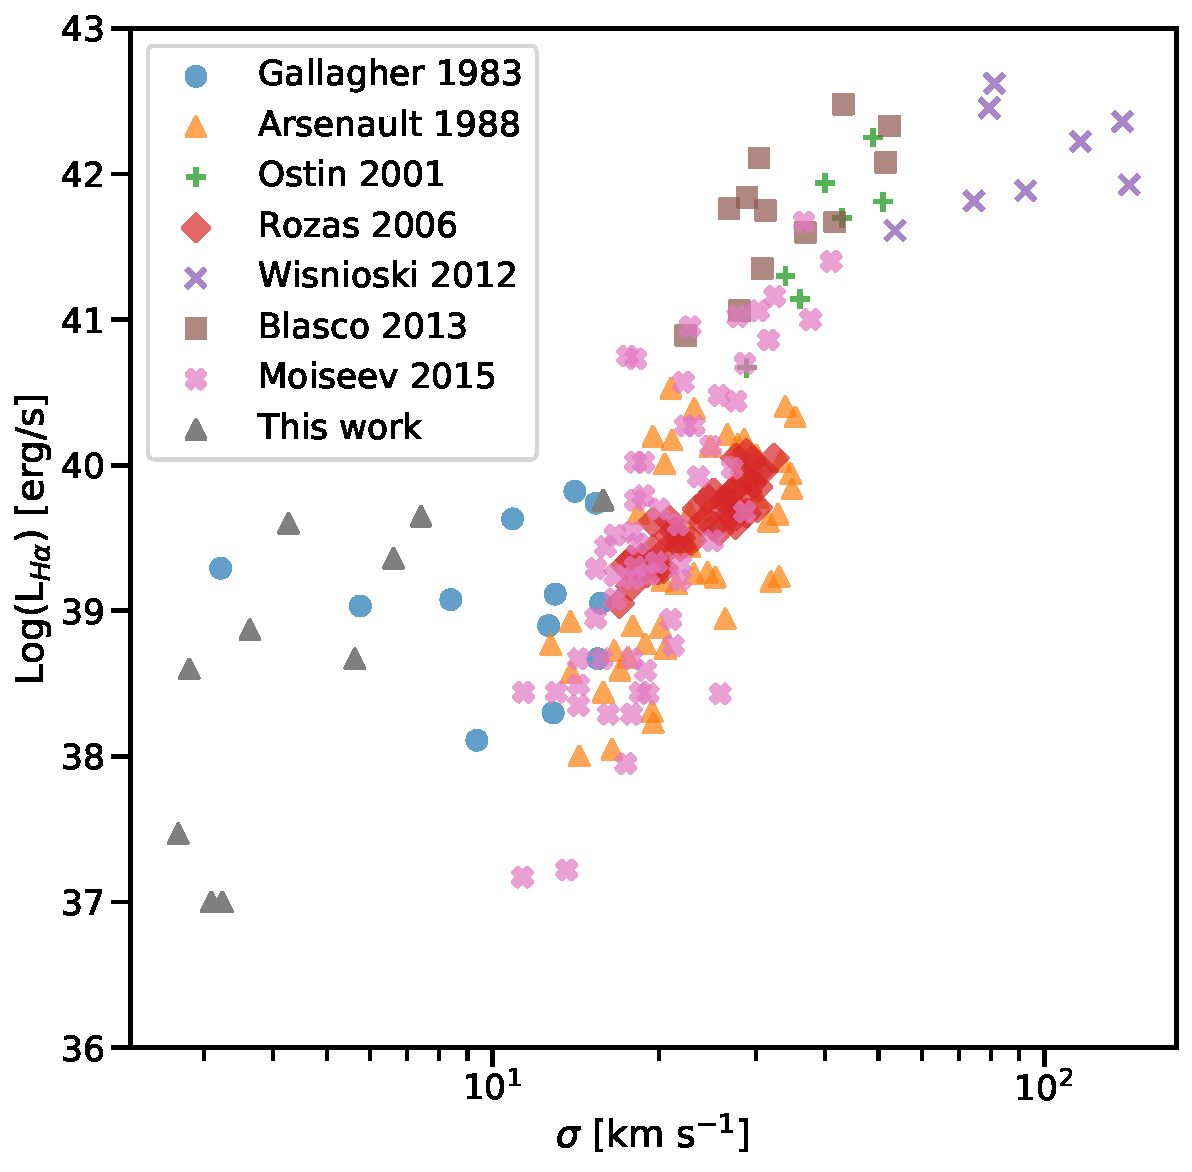
\includegraphics[width=3in]{Figures/lvss.pdf}
\caption{}
\label{fig:}
\end{figure}

%\begin{figure}
%\centering 
%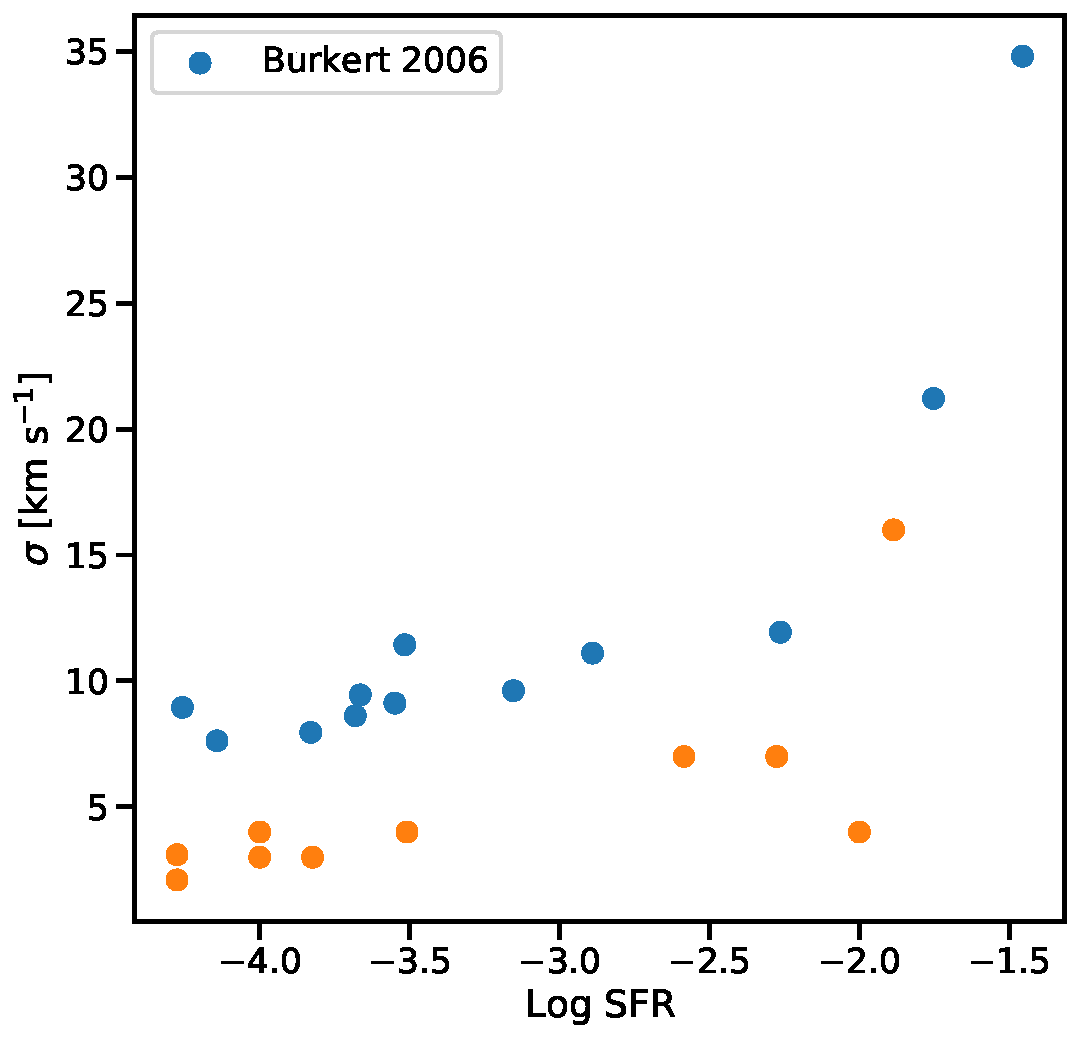
\includegraphics[width=3in]{Figures/sfrvssig.pdf}
%\caption{\citet{2006CRPhy...7..433B}}
%\label{fig:}
%\end{figure}


Relationship between plane-of-sky and line-of-sight velocity dispersion.
Comparison with \citet{Rozas:2006b}.

%%%%%%%%%%%%%%%%%%%%%%%%%%%%%%%%%%%%%%%%%%%%%%%%%%%%%%%%%%%%%%%%%%%%%%%%%%%%%%%%%%%%%%%%%%%%%%%%%%%%%%%%%%%%%%%%%%%%%%


\section{Conclusions}\label{sec:conclusions}

%\begin{enumerate}
%    \item The giant HII regions in  M 33, NGC 604 and NGC 595 shows an index of 1.7 and 1.55, respectively. 
    

    
%    \item The structure functions are presented for the first time for Hubble X and Hubble V, in NGC 6822. Hubble V shows and index of 1.65 and a correlation length of 3 pc, while Hubble X results are 1.6 and 4 pc.
    
%    \item The structure function of 30 Dor is presented for the first time using high-resolution observations that allows to observe scales $>$0.1 pc. A correlated structure function is obtained with a correlation lenght of 2.7 pc and a power-law index of 1.15. This new results show that previous studies on 30 Dor structure functions were analyzing large scales where no velocity fluctuations are present.

    
%\end{enumerate}

%%%%%%%%%%%%%%%%%%%%%%%%%%%%%%%%%%%%%%%%%%%%%%%%%%%%%%%%%%%%%%%%%%%%%%%%%%%%%%%%%%%%%%%%%%%%%%%%%%%%%%

\section*{Acknowledgements}

We are grateful to Norberto Castro Rodríguez for providing maps of emission line velocity moments for 30 Doradus derived from MUSE-VLT observations.

%%%%%%%%%%%%%%%%%%%%%%%%%%%%%%%%%%%%%%%%%%%%%%%%%%
%%%%%%%%%%%%%%%%%%%% REFERENCES %%%%%%%%%%%%%%%%%%

\bibliographystyle{mnras}
\bibliography{bibphd}

%\clearpage

%%%%%%%%%%%%%%%%%%%%%%%%%%%%%%%%%%%%%%%%%%%%%%%%%%
%%%%%%%%%%%%%%%%% APPENDICES %%%%%%%%%%%%%%%%%%%%%
%%%%%%%%%%%%%%%%%%%%%%%%%%%%%%%%%%%%%%%%%%%%%%%%%%

%\appendix

%\section{Velocity maps}\label{sec:VelMaps}

%\begin{figure*}
%\centering
%\begin{multicols}{4}
%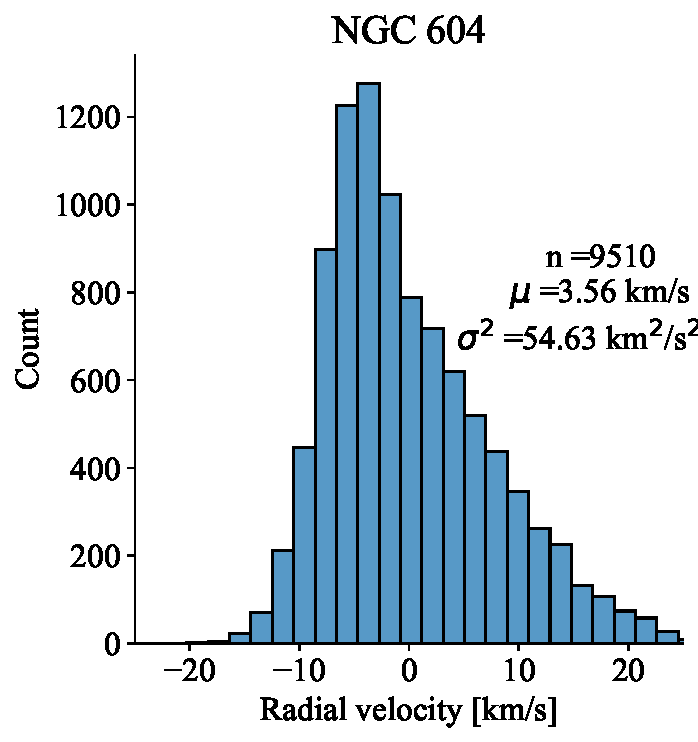
\includegraphics[width=1.5in]{Figures/Hist/604}\par
%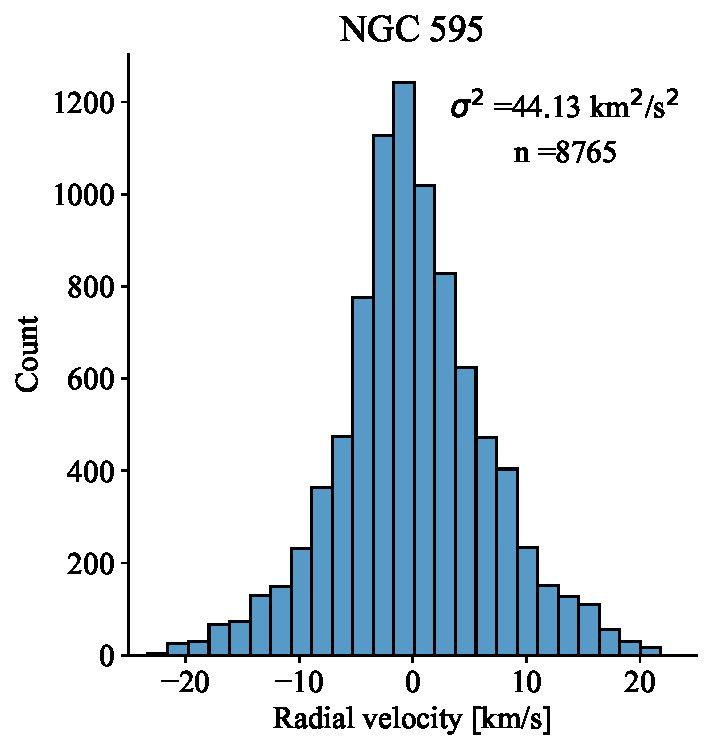
\includegraphics[width=1.5in]{Figures/Hist/595.pdf}\par
%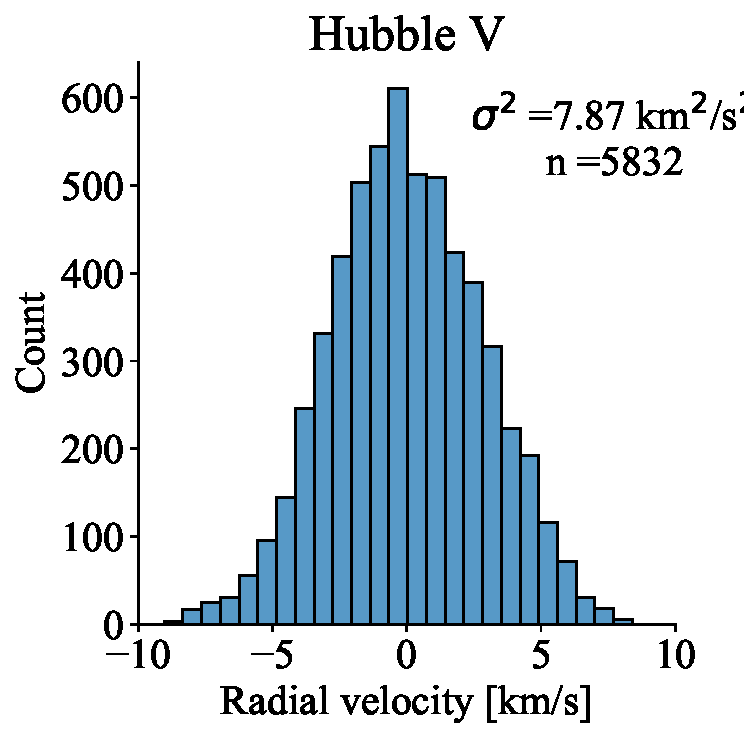
\includegraphics[width=1.5in]{Figures/Hist/Hubble V.pdf}\par
%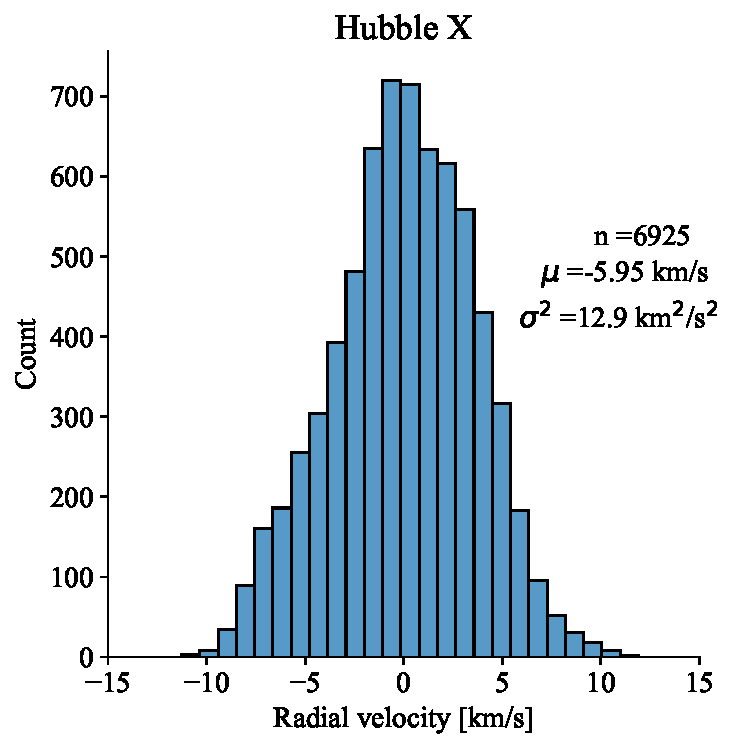
\includegraphics[width=1.5in]{Figures/Hist/Hubble X.pdf}\par
%\end{multicols}
%\begin{multicols}{4}
%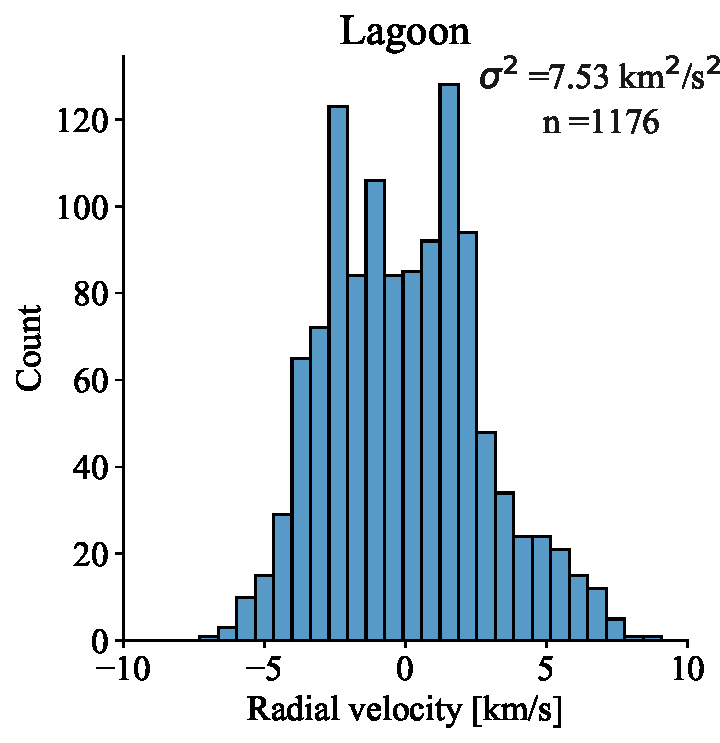
\includegraphics[width=1.5in]{Figures/Hist/M8.pdf}\par
%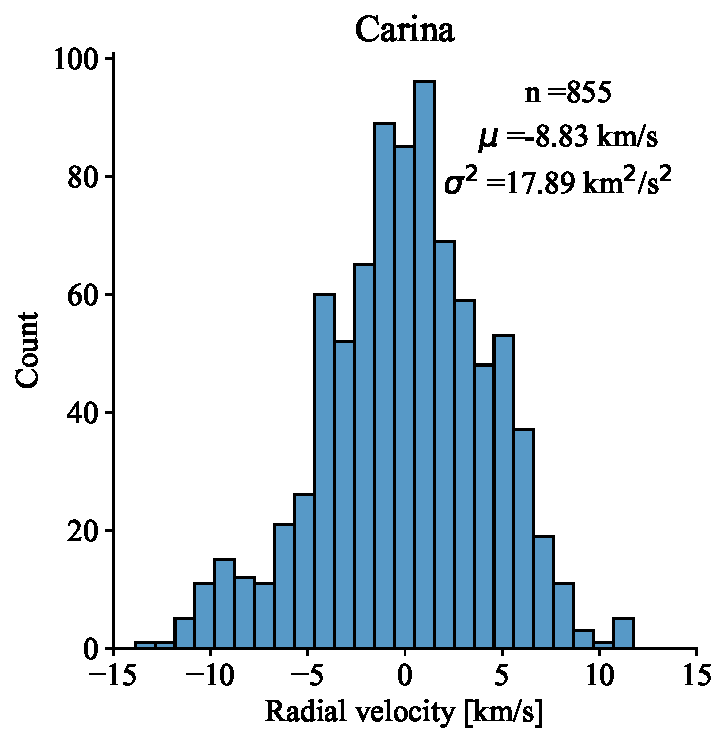
\includegraphics[width=1.5in]{Figures/Hist/Car.pdf}\par
%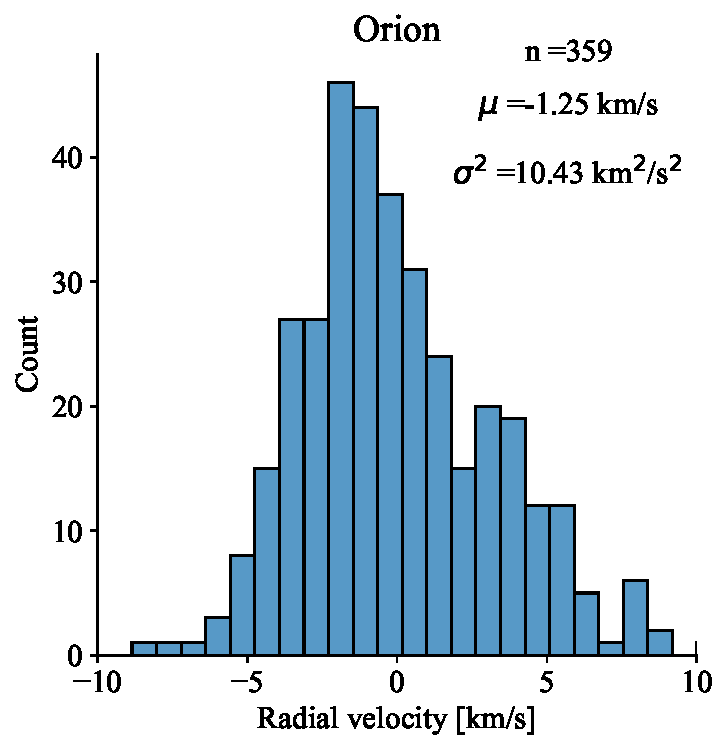
\includegraphics[width=1.5in]{Figures/Hist/Orion.pdf}\par
%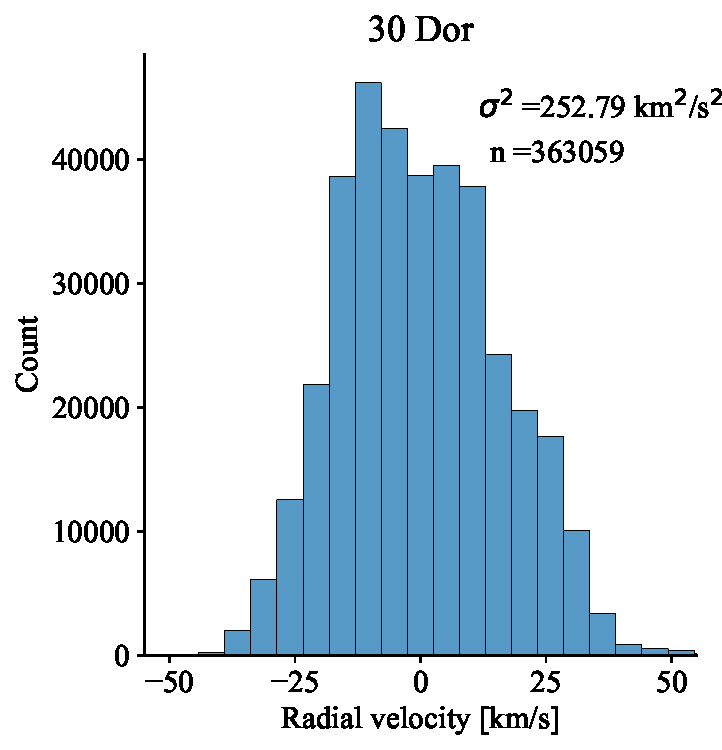
\includegraphics[width=1.5in]{Figures/Hist/30Dor.pdf}\par
%\end{multicols}
%\caption{}
%\label{fig:hist}
%\end{figure*}



%\begin{figure}
%\centering 
%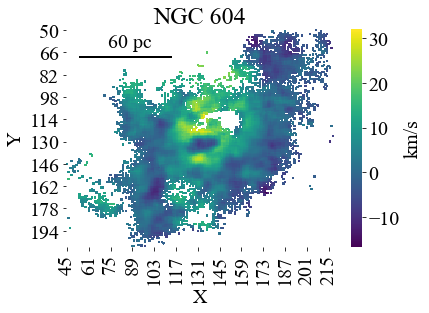
\includegraphics[width=2.5in]{Figures/M6T}
%\caption{Radial velocity maps of NGC 604 in H$\alpha$.  }
%\label{fig:M604}
%\end{figure}

%\begin{figure}
%\centering 
%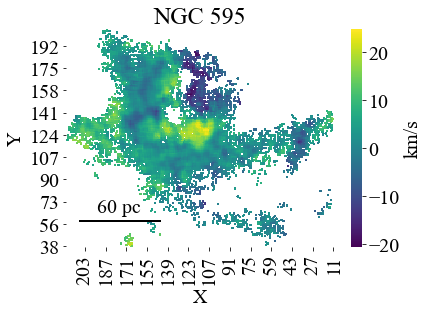
\includegraphics[width=2.5in]{Figures/M5T}
%\caption{Radial velocity map of NGC 595 in H$\alpha$.}
%\label{fig:M595}
%\end{figure}

%\begin{figure}
%\centering 
%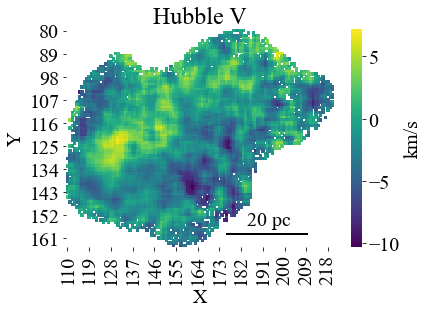
\includegraphics[width=2.5in]{Figures/MV}
%\caption{Radial velocity map of Hubble V in H$\alpha$.}
%\label{fig:MHV}
%\end{figure}

%\begin{figure}
%\centering 
%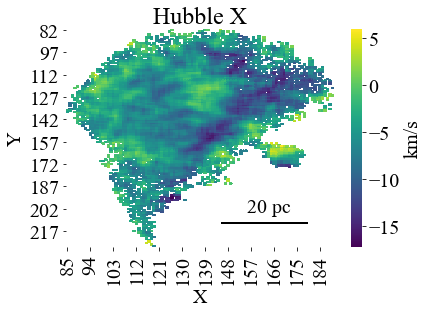
\includegraphics[width=2.5in]{Figures/MX}
%\caption{Radial velocity map of Hubble X in H$\alpha$.}
%\label{fig:MHX}
%\end{figure}

%\begin{figure}
%\centering 
%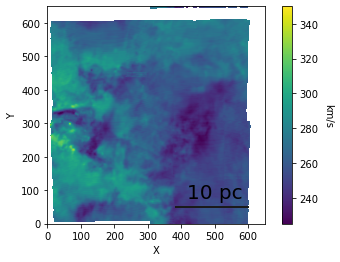
\includegraphics[width=2.5in]{Figures/M30D}
%\caption{Radial velocity map of 30 Dor in H$\alpha$ \citep{Castro:2018a}.}
%\label{fig:M30Dor}
%\end{figure}

%\begin{figure}
%\centering 
%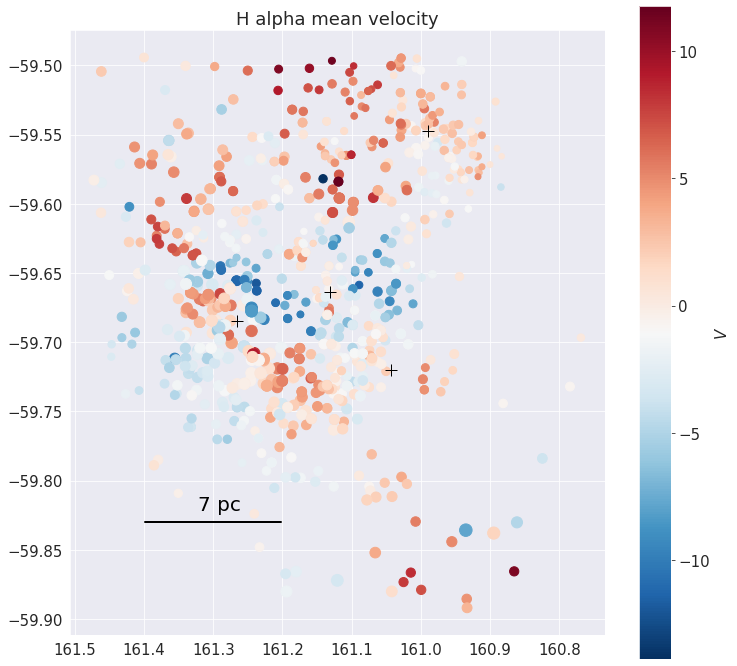
\includegraphics[width=2.5in]{Figures/Car}
%\caption{Radial velocity map of Carina in H$\alpha$ taken from \citet{Damiani:2016a}.}
%\label{fig:MCar}
%\end{figure}

%\begin{figure}
%\centering 
%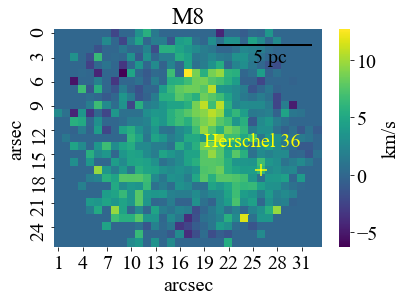
\includegraphics[width=3in]{Figures/M8H.png}
%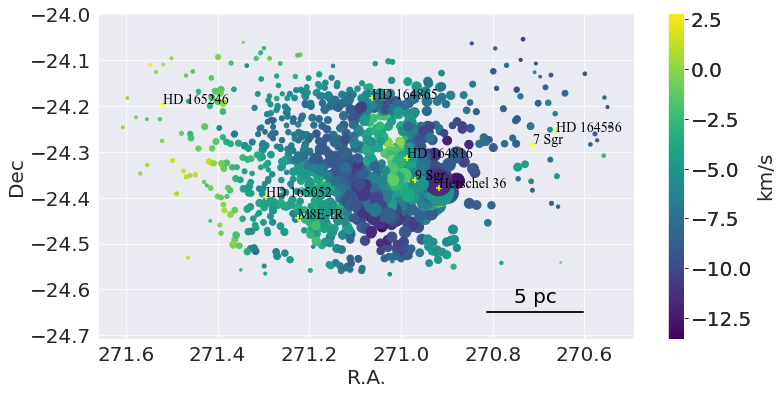
\includegraphics[width=3.5in]{Figures/M8}
%\caption{Radial velocity map of M8 in H$\alpha$. Taken from \citep{Damiani:2017b} and \citet{1987A&A...176..338H}.}
%\label{fig:MM8}
%\end{figure}

%\begin{figure}
%\centering 
%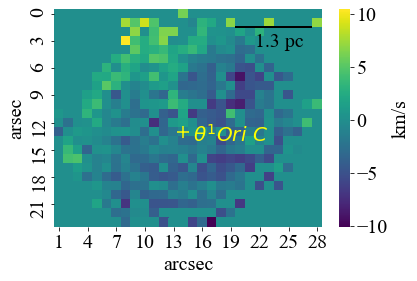
\includegraphics[width=3in]{Figures/OrionL}
%\caption{Radial velocity map of Orion in H$\alpha$ taken from \citet{1987A&A...176..347H}.}
%\label{fig:MOrion}
%\end{figure}

%\clearpage

%\section{Second order structure functions}\label{sec:StructFunct}

%Here we present the plots of the second order structure functions...

%\begin{figure}
%\centering 
%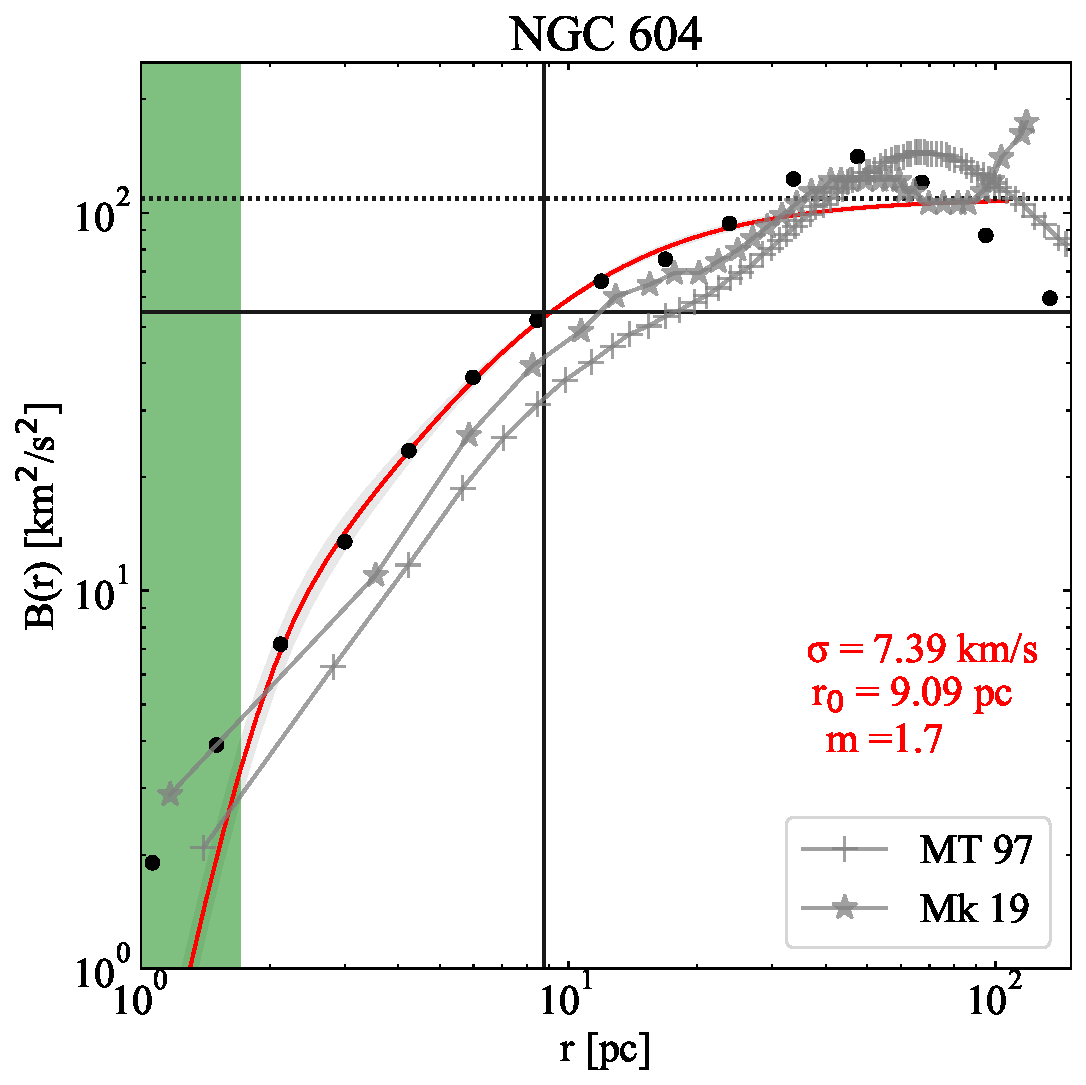
\includegraphics[width=2in]{Figures/SFplots/604}
%\caption{NGC 604 second-order structure functions for H$\alpha$ emission line from the ISIS and TAURUS instruments (Fig. \ref{}).
%The figure also shows the structure functions presented in previous works \citep{tanco1997,2019arXiv191203543M}.
%The green area represents the scales affected by observational seeing.
%The vertical line indicate the value of rhe correlation length , r$_{0}$.
%The solid horizontal line denote the value of $\sigma$.
%The double dotted horizontal line indicates 2$\sigma$.
%Black plots are structure functions calculated in this work and gray plots are from previous works.
%}
%\label{fig:SF604}
%\end{figure}

%\begin{figure}
%\centering 
%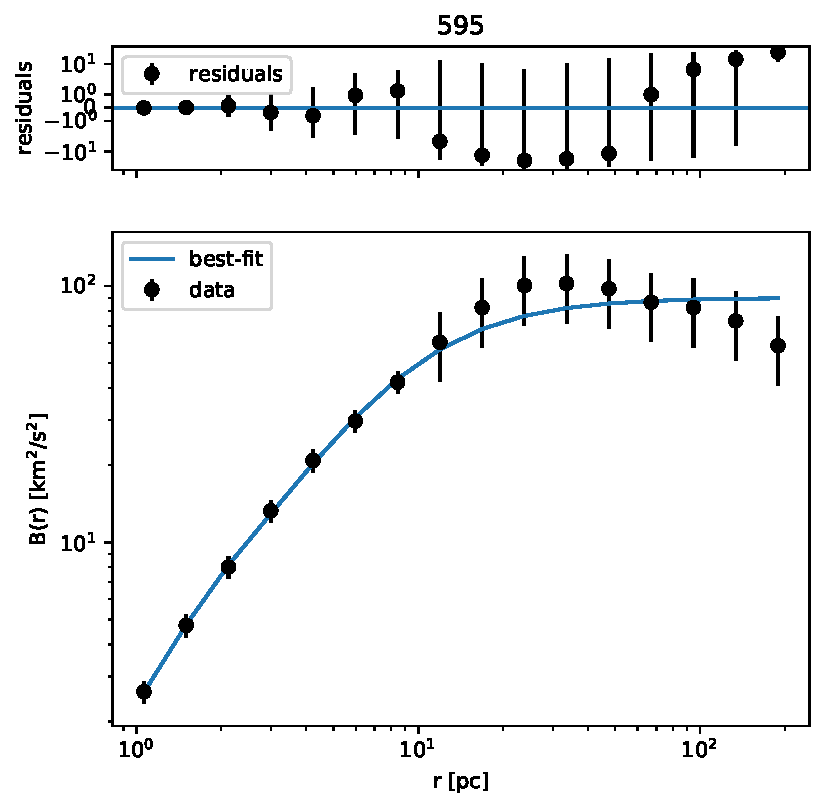
\includegraphics[width=2in]{Figures/SFplots/595}
%\caption{NGC 595 second-order structure functions for H$\alpha$ emission line from the TAURUS instrument (Fig. \ref{}).
%Same information as Figure \ref{fig:SF604}.}
%\label{fig:SF595}
%\end{figure}

%\begin{figure}
%\centering 
%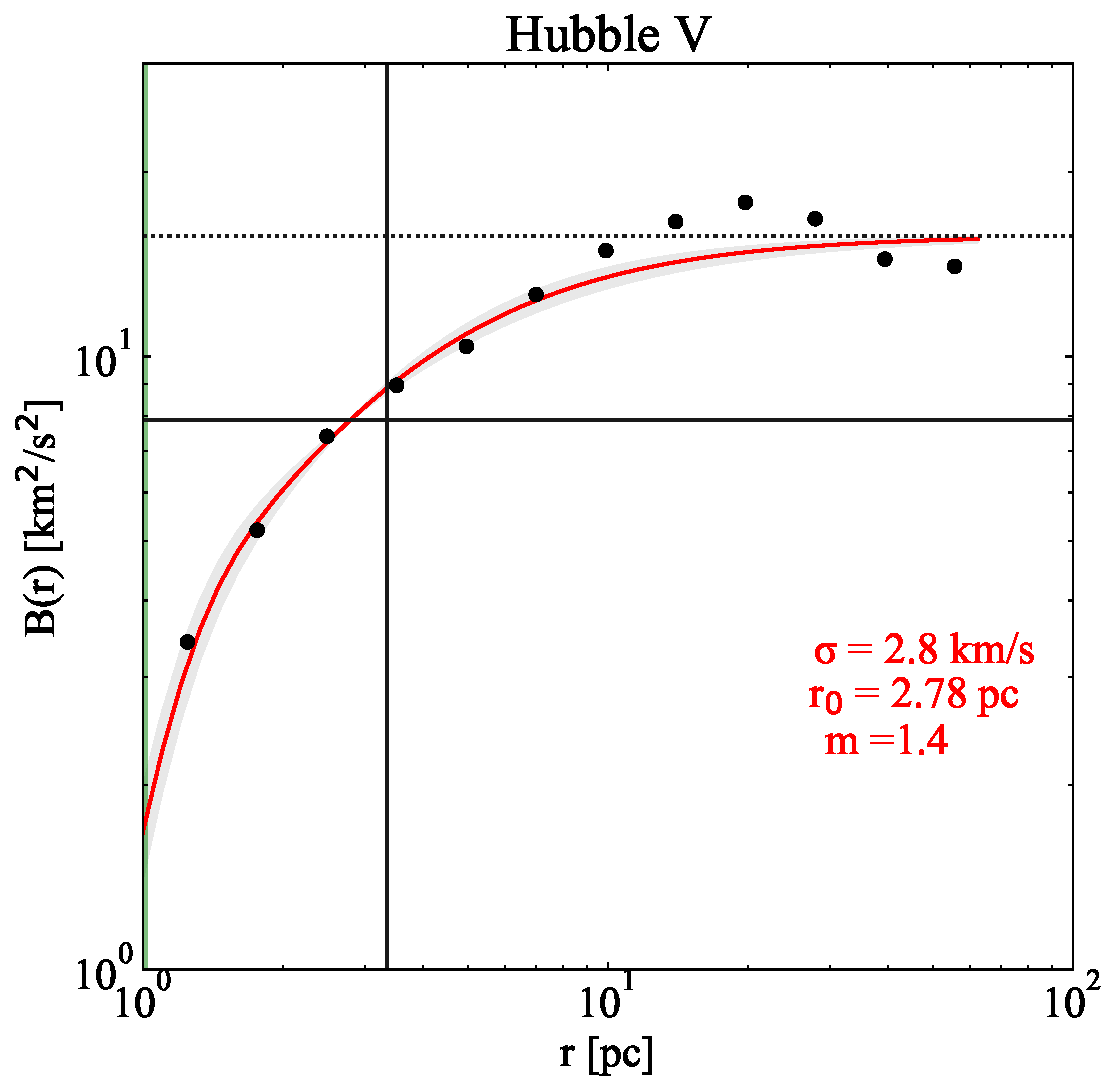
\includegraphics[width=2in]{Figures/SFplots/hubbleV}
%\caption{Hubble V second-order structure functions for H$\alpha$ emission line from the TAURUS instrument \ref{}).
%Same information as Figure \ref{fig:SF604}.}
%\label{fig:SFV}
%\end{figure}

%\begin{figure}
%\centering 
%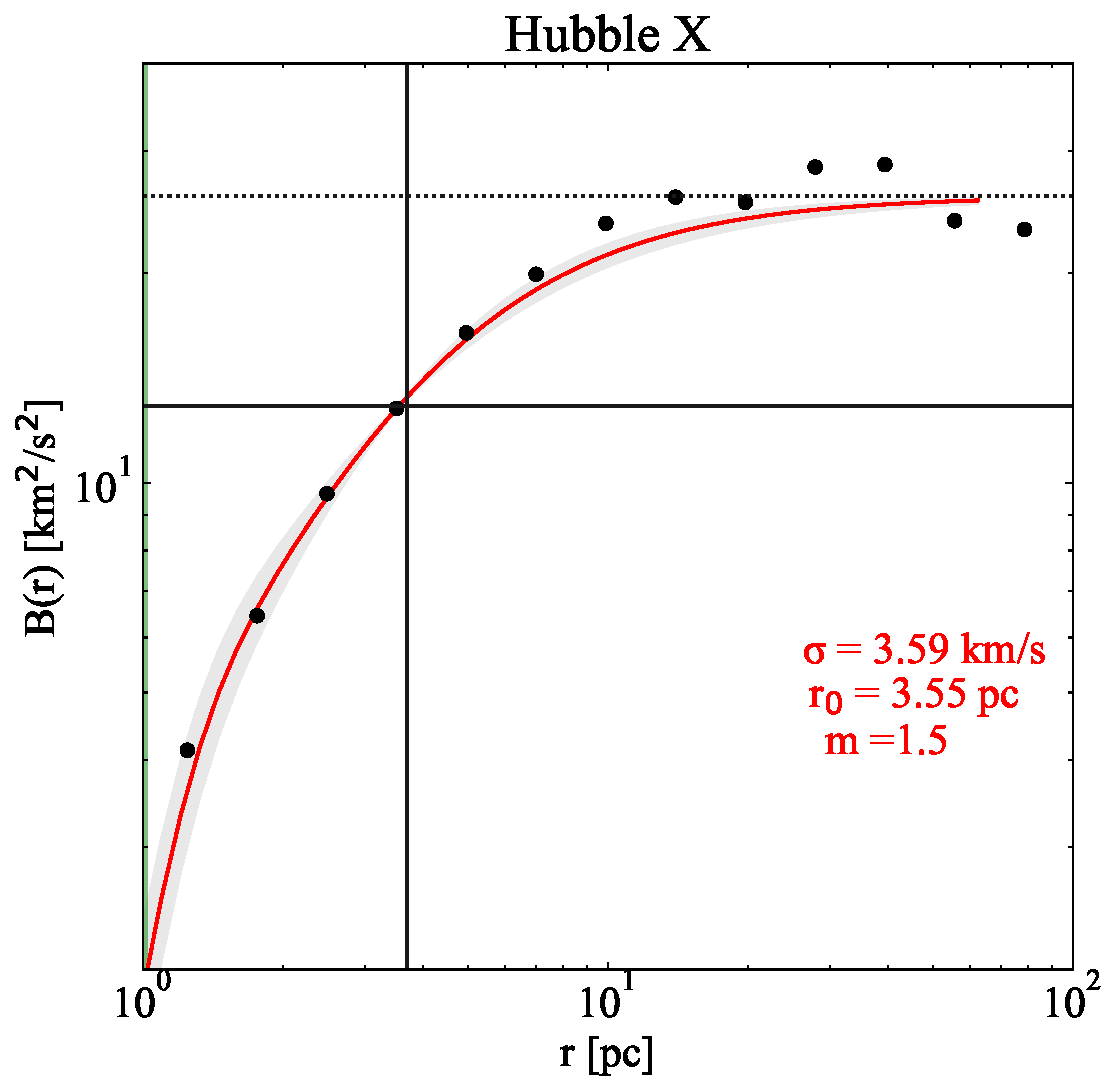
\includegraphics[width=2in]{Figures/SFplots/hubbleX.pdf}
%\caption{Hubble X second-order structure functions for H$\alpha$ emission line from the TAURUS instrument \ref{}).
%Same information as Figure \ref{fig:SF604}.}
%\label{fig:SFX}
%\end{figure}

%\begin{figure}
%\centering 
%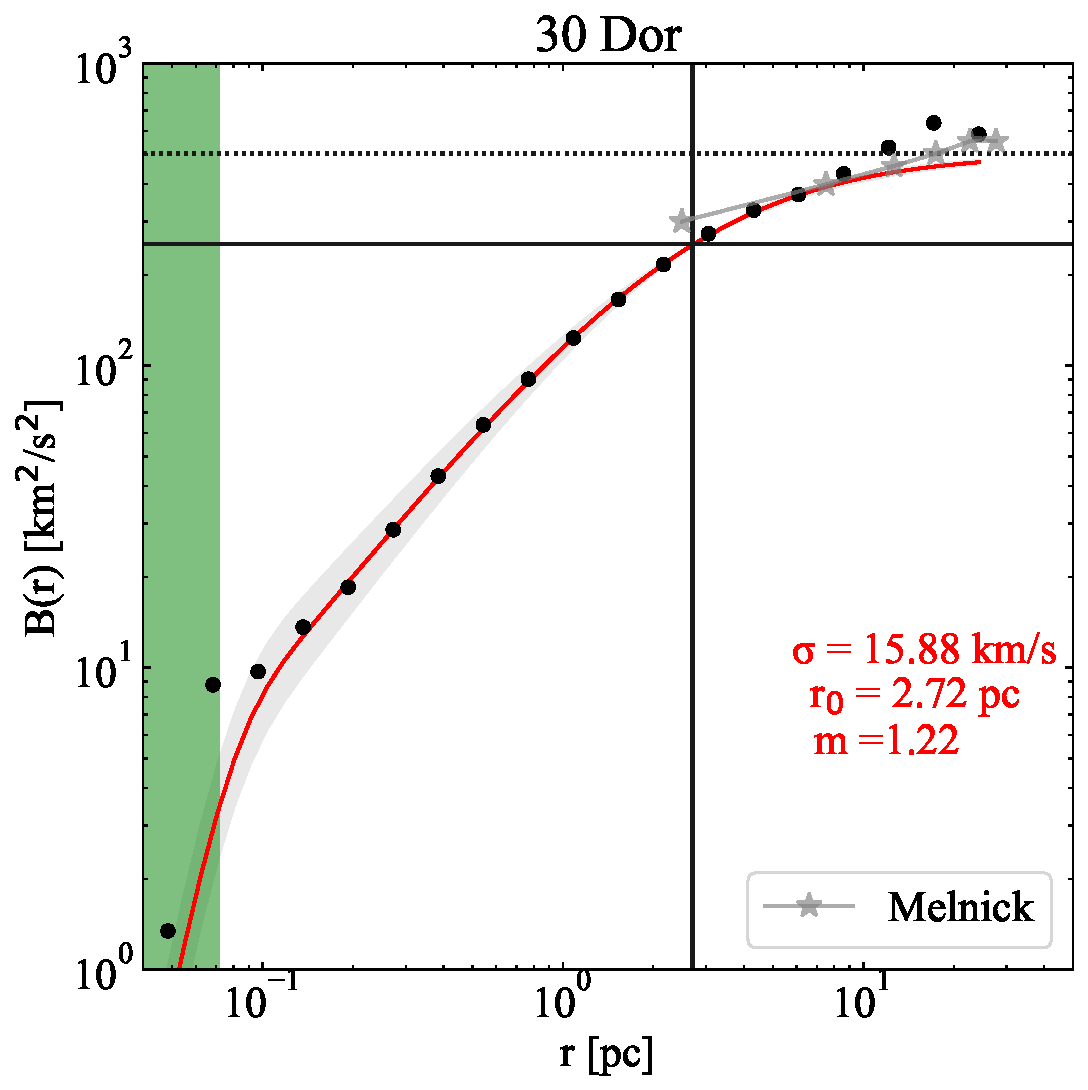
\includegraphics[width=2in]{Figures/SFplots/tarantula}
%\caption{30 Dor second-order structure functions for H$\alpha$ emission line \citep{Castro:2018a}.
%The figure also shows the structure functions presented in previous works \citep{2019arXiv191203543M}.
%Same information as Figure \ref{fig:SF604}.}
%\label{fig:SF30Dor}
%\end{figure}

%\begin{figure}
%\centering 
%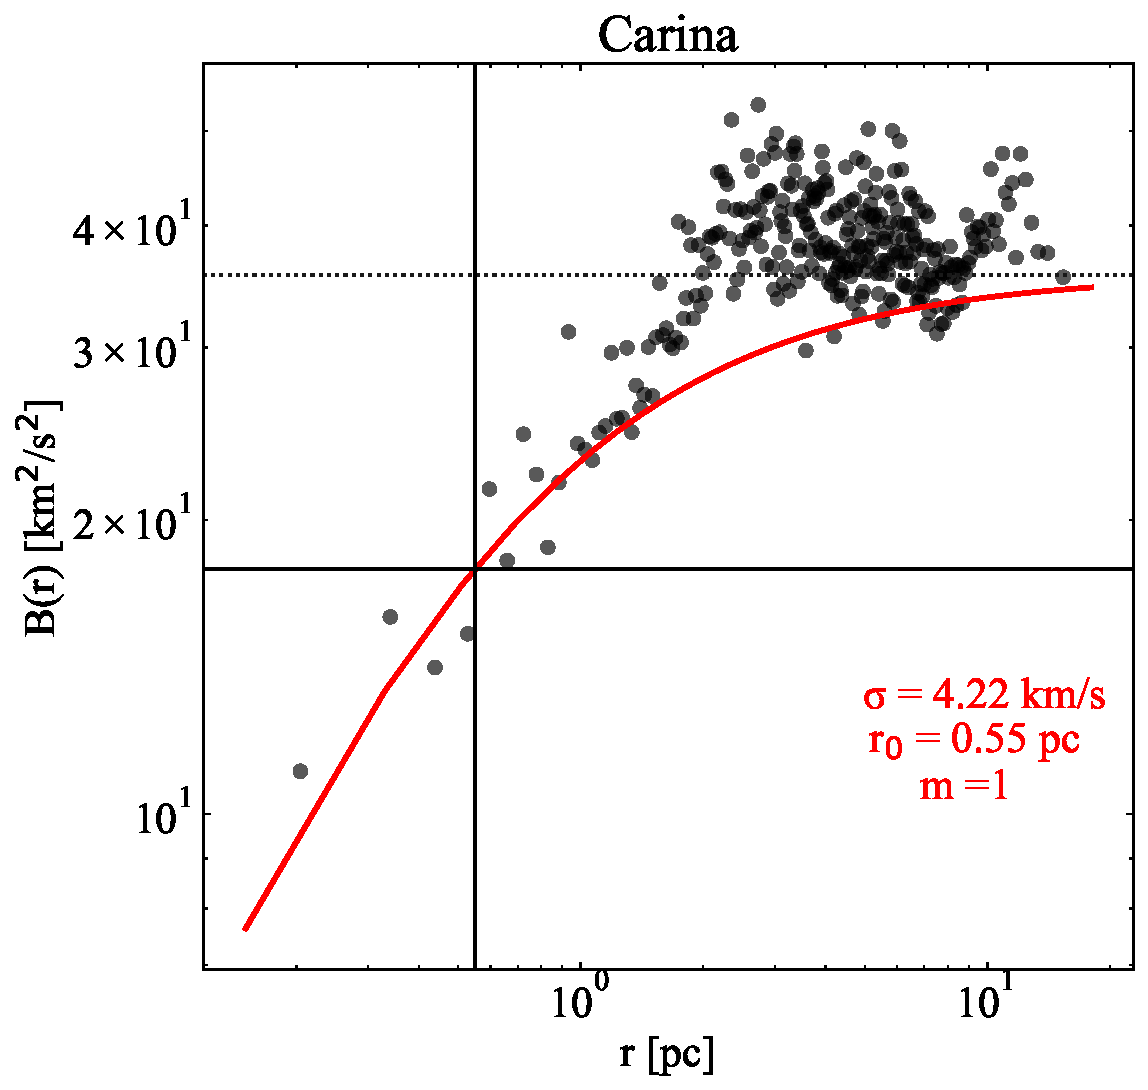
\includegraphics[width=2in]{Figures/SFplots/carina}
%\caption{Carina second-order structure functions for H$\alpha$ emission line taken from.
%Same information as Figure \ref{fig:SF604}.}
%\label{fig:SFCar}
%\end{figure}

%\begin{figure}
%\centering 
%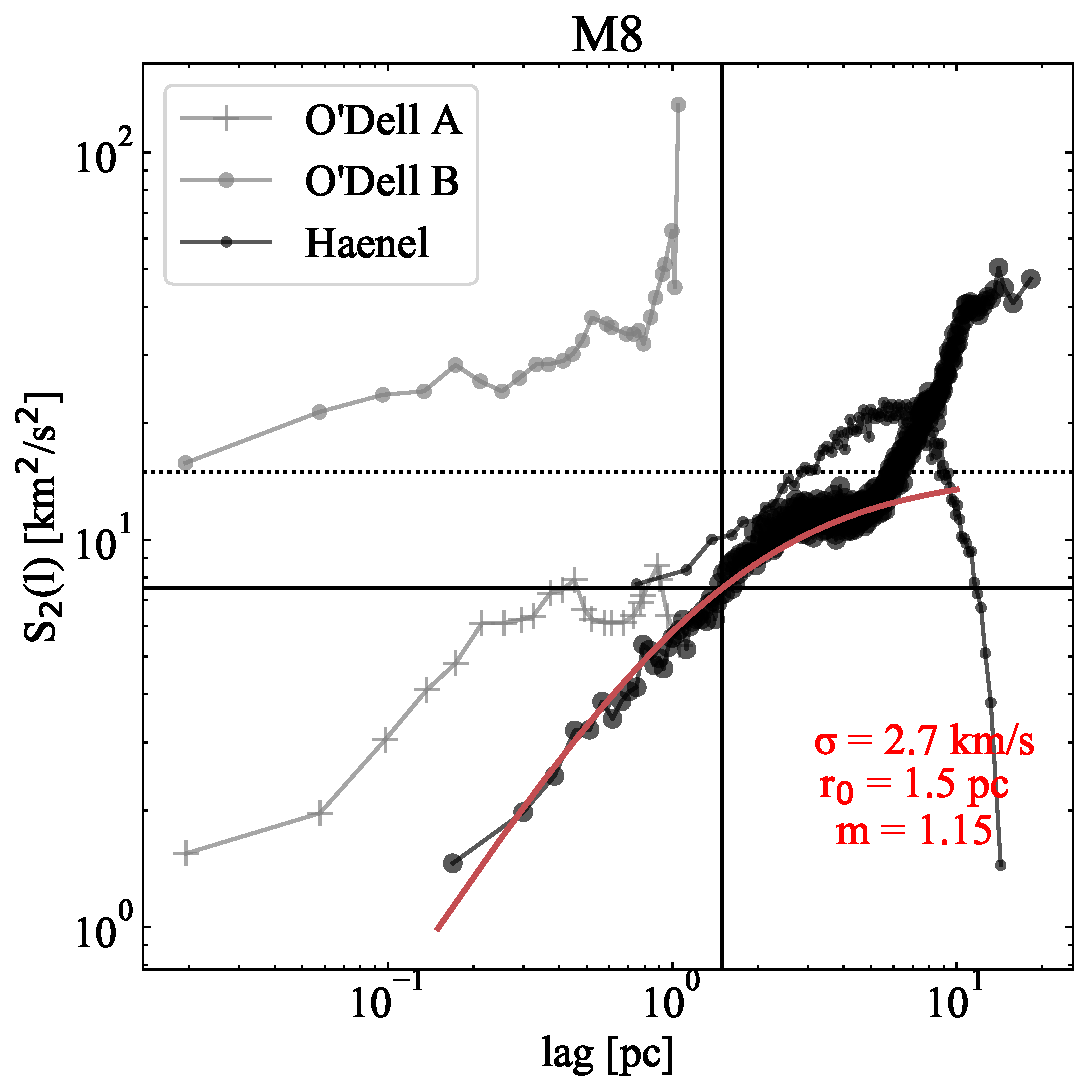
\includegraphics[width=2in]{Figures/SFplots/M8}
%\caption{M8 second-order structure functions for H$\alpha$ emission line \ref{}) from  \citet{Damiani:2017b} and \citet{1987A&A...176..338H}.
%The figure also shows the structure functions presented in previous works \citep{1987ApJ...317..686O}.
%Same information as Figure \ref{fig:SF604}.}
%\label{fig:SFM8}
%\end{figure}

%\begin{figure}
%\centering 
%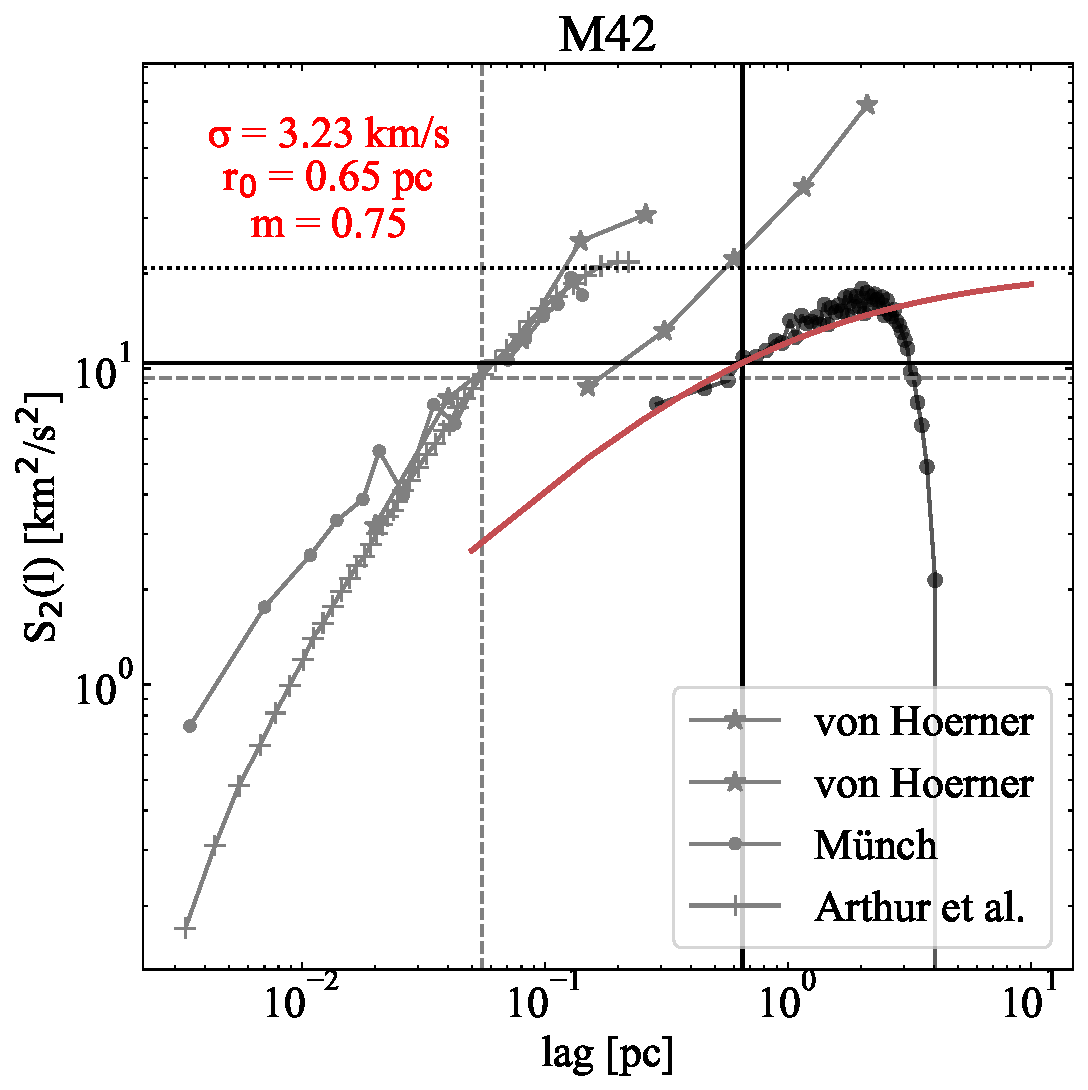
\includegraphics[width=2in]{Figures/SFplots/M42}
%\caption{M42 second-order structure functions for H$\alpha$ emission line taken from \citet{1987A&A...176..347H} \ref{}).
%he figure also shows the structure functions presented in previous works \citep{von1951methode,munch1958internal,arthur2016turbulence}.
%Same information as Figure \ref{fig:SF604}.}
%\label{fig:SFM42}
%\end{figure}




% Don't change these lines
\bsp	% typesetting comment
\label{lastpage}
\end{document}

% End of mnras_template.tex
%%% Local Variables:
%%% mode: latex
%%% TeX-master: t
%%% End:
